% ========================================================
% INTERPRETACIÓN DE LOS CLUSTERS Y CASO DE USO ODS 11
% ========================================================
\section{Interpretación de los clusters y caso de uso ODS 11}\label{sec:interpretacion-clusters}

La Sección~\ref{sec:caso} dejó planteada la pregunta central del caso de uso: \enquote{¿qué tipos
de viaje componen la movilidad en taxi amarillo de Nueva York, y cómo se distribuyen entre las zonas
de la ciudad?}. La PC2 postergó esa respuesta para priorizar la concurrencia y la medición del
speedup (Sección~\ref{sec:correcciones-pc2}). Este entregable cierra la pregunta analizando los
centroides del modelo final de K-means y su agregación espaciotemporal sobre los 2\,831\,486 viajes
del dataset limpio.

\subsection{Los ocho arquetipos de movilidad}

Con $K = 8$ y semilla 2024, la corrida canónica converge en la inercia \cifra{inercia-convergente}
(4\,461\,447{,}06). La Tabla~\ref{tab:clusters-resumen} presenta la interpretación semántica de cada
cluster a partir de sus centroides en las seis dimensiones de entrenamiento, transformadas a sus
unidades físicas reales (minutos, millas y velocidad comercial en millas por hora).

\begin{table}[H]
\caption{Arquetipos de viaje identificados por K-means ($K = 8$)}\label{tab:clusters-resumen}
\small
\begin{tabularx}{\textwidth}{@{}c L{3.8cm} r r r r L{2.2cm} Y@{}}
\toprule
\textbf{ID} & \textbf{Arquetipo} & \textbf{\%} & \textbf{Min.} & \textbf{Mi.} & \textbf{mph} & \textbf{Pico / Día} & \textbf{Función urbana} \\
\midrule
0 & Salida laboral y cena & 14{,}9\,\% & 7{,}9 & 1{,}2 & 9{,}1 & 19:30 Mié & Retorno a hogares y ocio vespertino \\
1 & Noche y ocio fin de semana & 12{,}7\,\% & 7{,}1 & 1{,}2 & 10{,}1 & 21:50 Sáb & Movilidad nocturna en Lower Manhattan \\
2 & Micro-salto de almuerzo & 13{,}3\,\% & 6{,}2 & 1{,}0 & 9{,}7 & 12:25 Lun & Diligencias corporativas en Manhattan \\
3 & Tráfico denso de negocios & 14{,}3\,\% & 17{,}0 & 2{,}3 & 8{,}1 & 12:05 Mié & Núcleo financiero a paso de congestión \\
4 & Retorno nocturno inter-borough & 12{,}2\,\% & 18{,}4 & 4{,}1 & 13{,}4 & 21:50 Mar & Cruce de puentes hacia Queens/Brooklyn \\
5 & Enlace aeropuerto y autopista & 10{,}8\,\% & 36{,}3 & 12{,}6 & 20{,}8 & 15:00 Mar & Conexión troncal con JFK y LaGuardia \\
6 & Paseo diurno fin de semana & 11{,}9\,\% & 16{,}2 & 2{,}4 & 8{,}9 & 15:05 Sáb & Turismo familiar, museos y parques \\
7 & Cierre rápido de semana & 9{,}9\,\% & 6{,}5 & 1{,}0 & 9{,}2 & 12:00 Vie & Última milla corporativa previa al descanso \\
\bottomrule
\end{tabularx}
\end{table}

Los arquetipos revelan una marcada partición funcional del transporte. Los viajes no varían de
forma continua, sino que se concentran en tres regímenes bien definidos:
\begin{enumerate}
  \item \textbf{Micro-desplazamientos de última milla (Clusters 2 y 7):} Trayectos de apenas 1{,}0
        milla y 6 minutos que representan el 23{,}2\,\% del total de viajes analizados.
  \item \textbf{Movilidad urbana en congestión (Clusters 0, 1, 3 y 6):} Trayectos de 1{,}2 a 2{,}4
        millas donde la velocidad comercial cae por debajo de 10~mph por saturación vial.
  \item \textbf{Corredores troncales y periféricos (Clusters 4 y 5):} Desplazamientos largos (4 a
        13 millas) por autopistas y puentes hacia otros distritos o terminales aeroportuarias, donde
        la velocidad media sube a 13--21~mph.
\end{enumerate}

\subsection{Distribución espaciotemporal y diagnóstico ODS 11.2}

La meta 11.2 del ODS~11 exige proporcionar acceso a sistemas de transporte seguros, asequibles y
sostenibles, reduciendo la dependencia vehicular evitable. La agregación por zona y franja horaria
muestra dos fenómenos empíricos de alto impacto para la planificación urbana:

\paragraph{Sustituibilidad peatonal en Manhattan central.} En Midtown Center (zona 161) al mediodía
laboral (12:00, lunes a viernes), la flota registra 6\,185 viajes por hora. Aunque el cluster
dominante por pluralidad es el Cluster~3 (44{,}7\,\% de dominancia, a paso de tortuga de 8{,}1~mph),
la suma de los Clusters~2 (24{,}0\,\%) y 7 (17{,}2\,\%) demuestra que \textbf{el 41{,}2\,\% de los
viajes (2\,550 viajes/hora) mide una milla o menos}. En distancias de 1\,600 metros en cuadrícula, la
caminata (12--15 minutos) o el uso de bicicletas compartidas (Citi Bike, 5--7 minutos) ofrecen
tiempos equivalentes o menores a los del automóvil atrapado en el tráfico corporativo. Este hallazgo
constituye una justificación empírica directa para la ampliación de ciclovías protegidas y la zona
de tarificación por congestión (\emph{CBD Tolling Program}).

\paragraph{Corredores aeroportuarios y asimetría de demanda.} El Cluster~5 (aeropuertos) alcanza su
pico de salidas a las 15:00 de días laborables. En los aeropuertos JFK (zona 132) y LaGuardia (zona
138), el Cluster~5 representa el 92{,}4\,\% (5\,742 viajes/h) y 90{,}8\,\% (4\,313 viajes/h) de los
viajes originados a esa hora. Simultáneamente, Manhattan genera a las 14:00 más de 7\,700 viajes
hacia aeropuertos (656 desde Midtown Center y 648 desde Times Square). Identificar estas zonas de
origen permite orientar a los operadores para evitar el rodaje vacío (\emph{deadheading}) y evaluar
servicios de buses lanzadera de alta capacidad desde estaciones troncales.

\begin{figure}[H]
\caption{Visualización espaciotemporal y análisis de arquetipos en dispositivo móvil}\label{fig:app-movil}
\centering
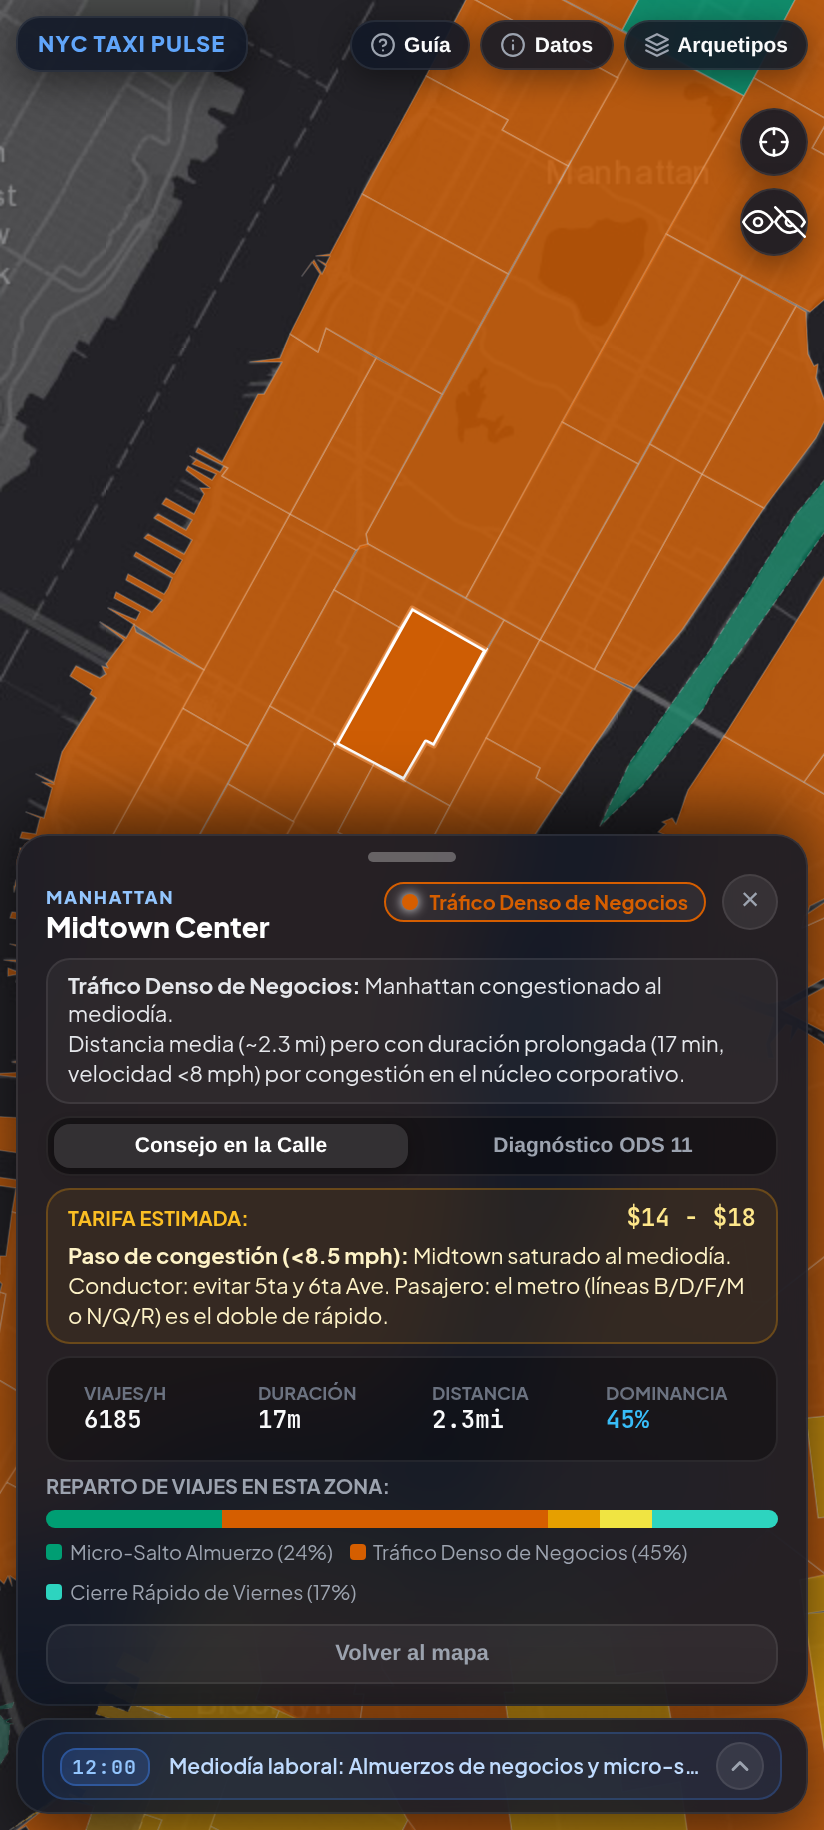
\includegraphics[width=0.42\textwidth]{img/app-movil-midtown.png}\hfill
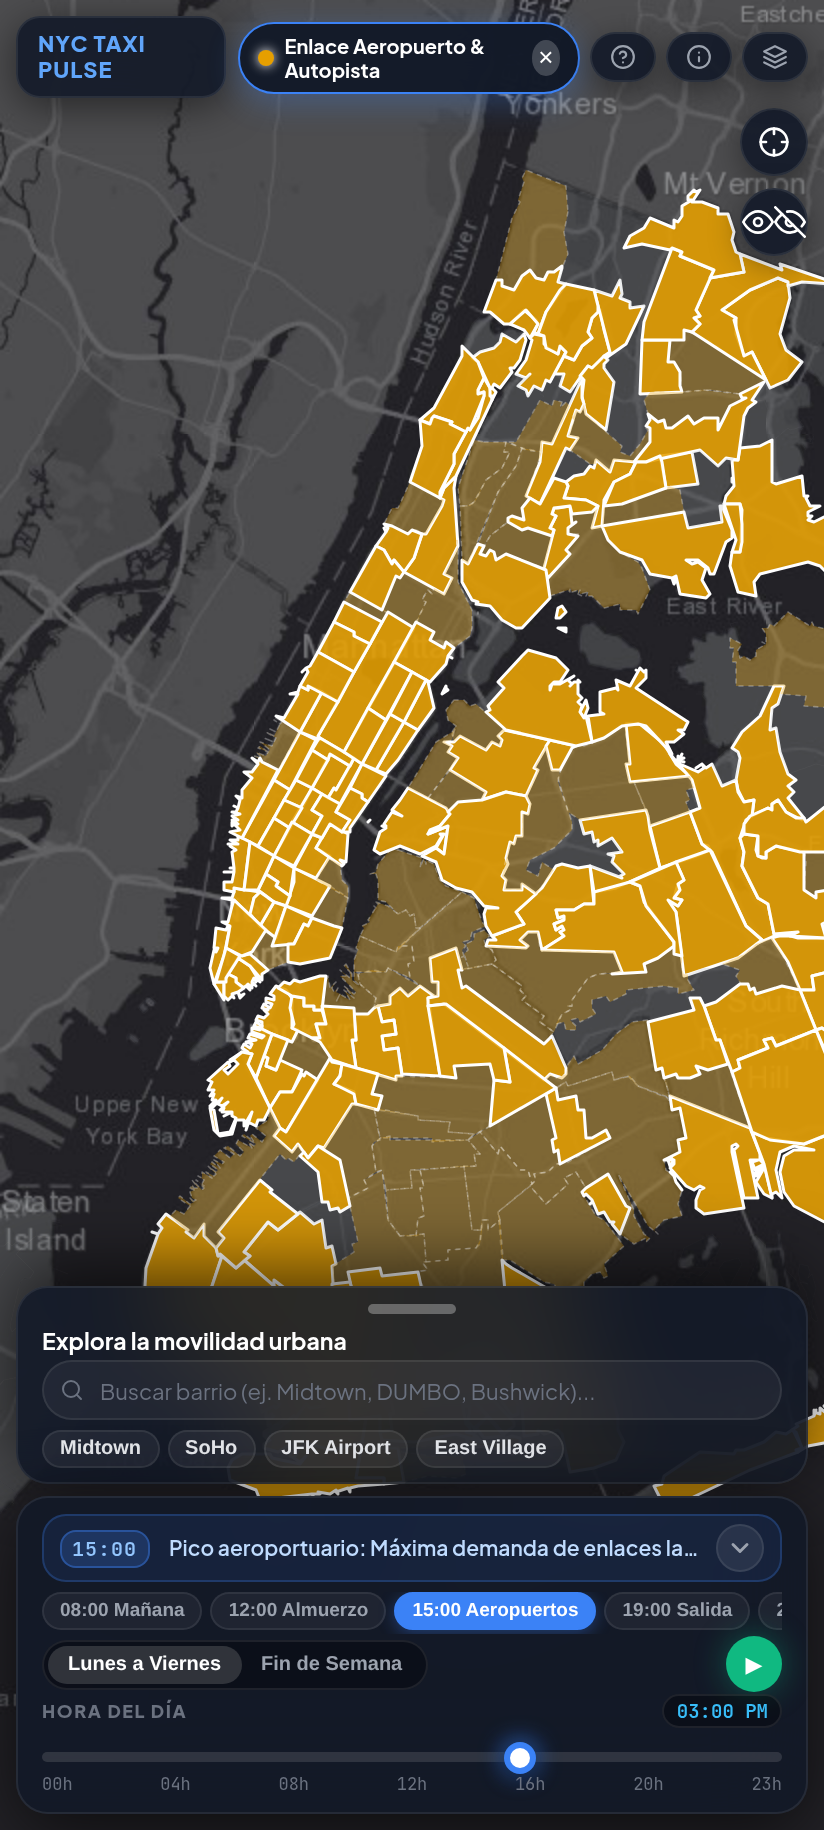
\includegraphics[width=0.42\textwidth]{img/app-movil-aeropuertos.png}
\caption*{A la izquierda, inspección de Midtown Center a las 12:00 con diagnóstico de congestión y
sustituibilidad peatonal (ODS 11.2). A la derecha, aislamiento del Cluster~5 (Aeropuertos) a las
15:00 evidenciando los corredores de salida de Manhattan y terminales aéreas.}
\end{figure}

\subsection{Herramienta de exploración y principio InWatch}

Para validar estos patrones de forma interactiva y sin sesgos estadísticos, el equipo desarrolló
un visualizador cartográfico ligero (\texttt{tp/app/}) con arquitectura desacoplada:
\begin{itemize}
  \item \textbf{Precómputo eficiente:} Un agregador en Go (\texttt{tp/kmeans/cmd/resumen\_zonas})
        procesa los 2{,}83 millones de asignaciones y genera un resumen compacto en formato JSON
        (735~KB), permitiendo una carga instantánea y funcionamiento \emph{offline} en navegadores
        móviles.
  \item \textbf{Principio de honestidad cartográfica (\emph{InWatch}):} Las zonas sin registros de
        taxis amarillos (10 de las 263 zonas de la TLC, como Freshkills Park o islas periféricas) no
        se interpolan ni se ocultan; la interfaz las declara explícitamente como áreas servidas por
        transporte público masivo (Metro MTA) o flotas locales. Asimismo, las franjas con muestra
        estadística reducida ($< 8$ viajes/hora) se representan con tramas discontinuas y alertas de
        flujo ligero.
  \item \textbf{Diseño centrado en el humano (HCD):} La interfaz fue evaluada con perfiles de
        usuario representativos (conductores, turistas y analistas de transporte), incorporando
        búsqueda predictiva de zonas, visualización de tarifas estimadas y paneles diferenciados
        para operación en calle y análisis de políticas públicas.
\end{itemize}
